
In this chapter several examples are shown of extraction of results
from the model output. The examples are again in the context of the
Madrid Metro as in the previous two chapters.

In the following, a time interval will be specified in the same way as
was done for calibration in \Chapref{Chap:MadCali}; a starting time and
ending time will be specified. This is sufficient for some overall
measurements.

In order to perform comparisons, the notion of \emph{comparable} from
\Secref{DefObj} is used; a number of sub-intervals will be
specified, and a quantity of interest will be averaged within each of
these sub-intervals. This will be used, for example, in describing the effect of a
disruption in \Secref{sec:incident}.

\section{Travel-time distribution}

As before, the travel-time distribution over all travelled
origin-destination pairs is taken to be a canonical measure of the
performance of the metro system. The distribution could be extracted for
a list of any subset of origin stations $\cal O$, any subset of
destination stations $\cal D$, and any time interval during the day.

For the system as a whole, for the whole day, the distribution is shown in \Figref{_TTDist2}
\begin{figure}[!ht]
  \centering
  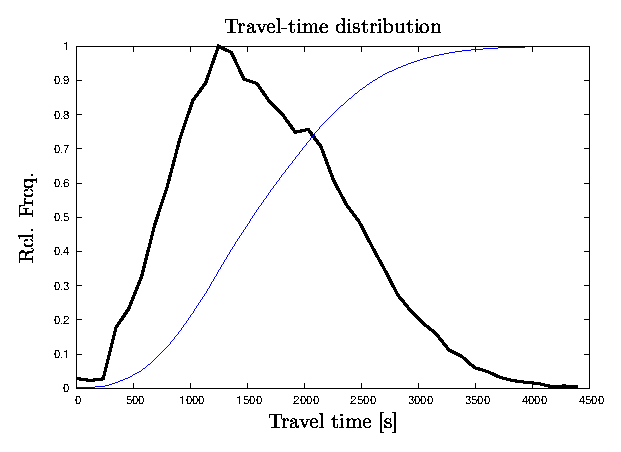
\includegraphics[angle=0,width=10cm]{90_figs/_TTD_0500-2500.eps}
  \caption{Distribution of travel time; $\mu=2333$ s, $\sigma=998$ s.}
  \label{_TTDist2}
\end{figure}

\section{Platform occupancy}

Platform occupancy appears in the simulation report as the number
of \zobj{zboxen} located inside a \zobj{zbox} of type Platform,
whenever entered by a passenger.

A script is provided to extract and collect these data from report lines.
To extract the occupancy at a given platform, say {\tt DEL\_Pf\_L10\_1}, as
a function of time,\\
\comline{./05\_FindPlatformOccupancy DEL\_Pf\_L10\_1 out/madrid\_08.zo} \\
The result is shown in \Figref{PlatOccup} for a portion of the morning.
\begin{figure}[!ht]
  \centering
  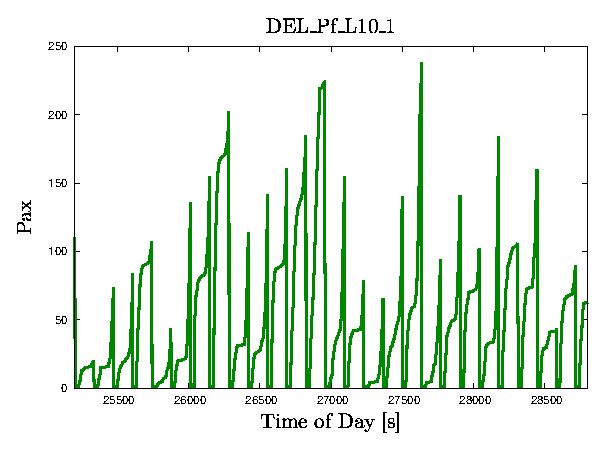
\includegraphics[angle=0,width=10cm]{90_figs/_Occupancy_DEL_Pf_L10_1.eps}
  \caption{Passengers waiting at DEL\_Pf\_L10\_1 from 07:00 to 08:00}
  \label{PlatOccup}
\end{figure}
The sawtooth shape is as expected; passengers arrive at the platform
over time, and leave together on a train. The intervals with zero
count are the dwelling intervals of a train; passengers do not
accumulate on the platform when a train is present.

\section{Train occupancy}
\begin{figure}[!ht]
  \centering
  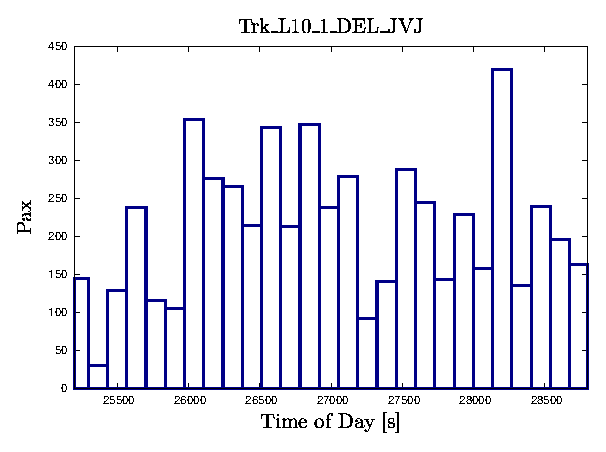
\includegraphics[angle=0,width=10cm]{90_figs/_Occupancy_Trk_L10_1_DEL_JVJ.eps}
  \caption{Passengers on trains leaving DEL\_Bn\_L12\_0 on Trk\_L10\_1\_DEL\_JVJ, during the interval from 07:00 to 08:00}
  \label{TrainOccup}
\end{figure}
Train occupancy, when leaving a platform (in fact the
{\tt Train} \zobj{zbox} leaves a {\tt Bound} \zobj{zbox}), appears in the
simulation report as the number of \zobj{zboxen} located inside
a \zobj{zbox} of type {\tt Train}, whenever this container enters
a \zobj{zbox} of type {\tt Track} (after having left a {\tt Bound}).

To instead extract train occupancy when arriving at a platform, it is necessary to
consider entry to the {\tt Bound} \zobj{zbox} rather than the following {\tt Track} \zobj{zbox}.

A script is provided to extract and collect these data from report lines.
To extract the occupancy of trains leaving a given platform, say {\tt DEL\_Bn\_L12\_0},
the track segment {\tt Trk\_L10\_1\_DEL\_JVJ} is identified: \\
\comline{./05\_FindTrainOccupancyAt Trk\_L10\_1\_DEL\_JVJ out/madrid\_08.zo} \\
The result is shown in \Figref{TrainOccup}.

Similarly, the occupancy of a train during its path through the system can be extracted.\\
\comline{./05\_FindRunningTrainOccupancy Train\_proto/L3/2 out/madrid\_08.zo} \\
The result is shown in \Figref{SingleTrain}. 
\begin{figure}[!ht]
  \centering
  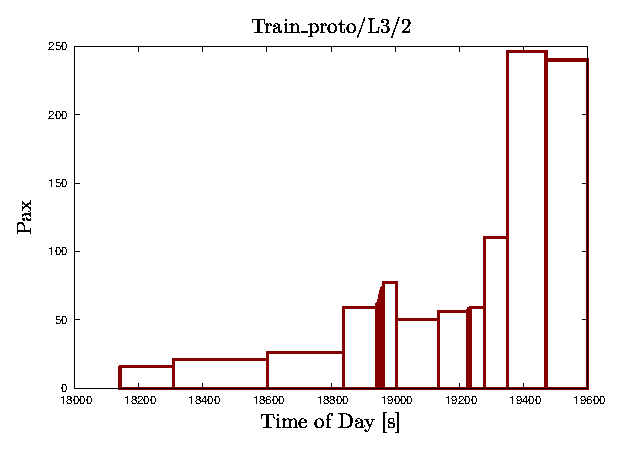
\includegraphics[angle=0,width=10cm]{90_figs/_Occupancy_Train_proto_L3_2.eps}
  \caption{Passenger count on single train Train\_proto/L3/2}
  \label{SingleTrain}
\end{figure}

\section{An event and consequences}
\label{sec:incident}
One way to simulate a blockage of a track is simply to insert a slow-moving blockage
in the desired track \zobj{zbox}, using input like the following, which
can be found in \\{\tt ZimInput/08\_BlockedTrackIncident.zim}.
\begin{lstlisting}[mathescape]
[zbox Blockage A=Train n=1 v=1.7 ]
[zbox BlockageWaitingRoom A=TrainSource n=1]
[zlink $\mu$=<BlockageWaitingRoom> $\nu$=<Trk_L10_1_DEL_JVJ> A={ Train . 1 } ]
[zlink $\mu$=<Trk_L10_1_DEL_JVJ> $\nu$=<BlockageSink> A={ Train . 1 } ]
[zbox BlockageSink A=TrainSink n=1]
[zschedule Deploy_Blockage
 S = [zsource $\phi$=<Blockage> m=One o=Teleport ]
 P = [zpath A=Train n=1 m=Open $\Lambda$={ [zstop $\phi$=<BlockageWaitingRoom>]
     [zstop $\phi$=<Trk_L10_1_DEL_JVJ>] [zstop $\phi$=<BlockageSink>] } ]
 T_0=0 T={ 07:30 } ]
\end{lstlisting}

At 07:30 the blockage is shifted into the track between DEL and JVJ stations.
The velocity is specified such that the track is blocked by this `Train' for 6 minutes.
The simulation including blockage can be run with
\comline{./08\_AddIncident\_RunSimulation.sh} \\
which will also produce a TTD analysis file using the Travel-time tool.
The travel-time distributions are shown in \Figref{TTD_comparison}.
\begin{figure}[!ht]
  \centering
  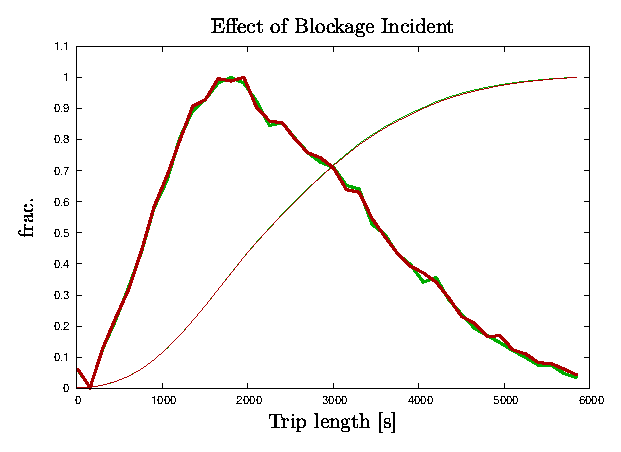
\includegraphics[angle=0,width=10cm]{90_figs/_TTD_incident_comparison.eps}
  \caption{Comparison of global travel-time distribution for base case (green) and incident (blockage) case (red):
  The distribution is for trips originating between 05:00 and 10:00, and the blockage is active from
  07:30 to 07:50. The blockage has no measurable effect in terms of this global distribution.}  
  \label{TTD_comparison}
\end{figure}

Although the effect of the incident is not significant in terms of the
travel-time distribution, it can be measured in terms of total
travel-time cost, measured in Passenger-seconds. With no incident, for
trips beginning within the interval 05:00-10:00, $2180644293$
passenger-seconds are reported by the travel-time tool; in the
incident case, $2183288493$. Therefore, the cost of this delay on the
line between DEL and JVJ stations is determined to be $(2183288493 -
2180644293)/3600 = 734$ passenger-hours.\footnote{No attempt here is
made to ascertain the standard deviation or other properties of this quantity; the present
goal is to illustrate extraction of data from simulation output.}

The effect of the incident is most obvious when platform and train
occupancies are compared with the base case without
incident. In \Figref{PlatOccupInc} is shown this comparison for the
downstream JVJ platform and trains leaving DEL. It is clear that in
the incident case, trains which have been held back and arrive more
closely in time after the incident is over are underutilised by
passengers.

\begin{figure}[!ht]
  \centering
  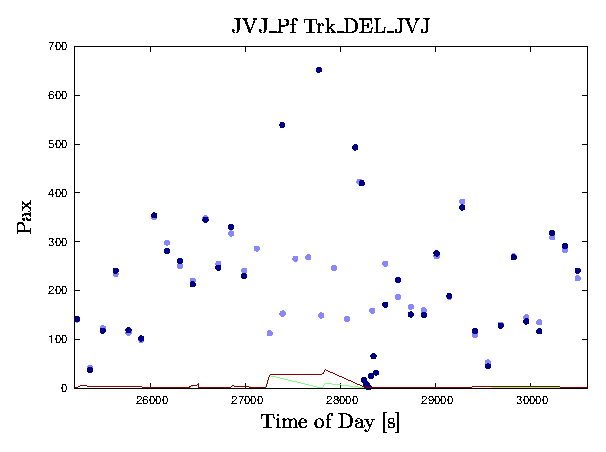
\includegraphics[angle=0,width=10cm]{90_figs/_Occupancy_JVJ_Pf_L10_1_and_Trk_to_JVJ_incident.eps}
\caption{Passengers waiting at JVJ\_Pf\_L10\_1 and riding on trains to this platform, from 07:00 to 08:30:
  The base case platform crowd is plotted in green, the incident case
  in red. The incident begins at 07:30 = 27000 s.  Train occupancy in
  the base case is plotted in light blue, the incident case in dark
  blue.  It is noted that the results even before the incident are not
  identical, due to the stochastic sampling of passenger walking
  speeds.  }
\label{PlatOccupInc}
\end{figure}

